\documentclass[12pt]{article}
\usepackage[utf8]{inputenc}
\usepackage{amsmath,amssymb}
\usepackage{unicode-math}
\usepackage[T2A]{fontenc}
\usepackage[russian]{babel}
\usepackage{graphicx}
\usepackage{subfigure}
\usepackage{subcaption}
\usepackage{url}


\DeclareGraphicsExtensions{.pdf,.png,.jpg}
\usepackage{hyperref}
\usepackage{wrapfig}
\usepackage[left=20mm, top=20mm, right=10mm, bottom=20mm]{geometry}

\usepackage{amsmath} 
\usepackage{amsfonts} 
\usepackage{amssymb} 
\usepackage{wasysym} 
\usepackage{fancyhdr}

\pagestyle{fancy}
\fancyhf{}
\lhead{Семинар 8. Эффект Зеемана. Правила отбора}
\rhead{\textit{Клименок К.Л., МФТИ 2020}}
\rfoot{\thepage}



\begin{document} 
\title{\textbf{Семинар Семинар 8. Эффект Зеемана. Правила отбора}}
\author{\textbf{Клименок Кирилл Леонидович}}
\date{30.09.2020}
\maketitle
\section{Теоретическая часть}
На данный момент мы с вами разобрались с устройством уровней энергии в разных сложных атомах, поняли, что такое спин и даже научились (надеюсь) писать термы различных энергетических состояний атома. Пришло время перейти к переходам между различными уровнями и поведении этих уровней энергии во внешнем магнитном поле.\\
Мне кажется, что уже становится понятно, если мы включим внешнее магнитное поле в выделенном направлении, то из-за проекции полного магнитного момента атома на это направление каждый уровень начнет расщепляться по энергиям, это приведет к еще большей сложности в строении уровней (эффект Зеемана) и к куче разных переходов между ними. А вот тут оказывается, что все не совсем однозначно. Некоторые переходы оказываются невозможны в силу правил отбора. Давайте про них и поговорим перед эффектом Зеемана
\subsection{Правила отбора}
\paragraph{Четность} Начнем с понятия четности и ее оператора. Вы конечно знаете про правые и левые тройки векторов в трехмерном пространстве, и что одна из них является зеркальным отражением другой. Можно ли тогда ввести  оператор инверсии, который бы зеркально транслировал наше обычное пространство в зеркальное. Да, разумеется, это делается очень легко, такой оператор называется оператором четности: $\hat{\mathfrak{p}}$ (я буду использовать готическое начертание, чтобы не путать с импульсом) все что он делает -- это изменение вектора координаты $\textbf{r} \rightarrow -\textbf{r}$. Давайте найдем собственные значения этого оператора, просто применив его 2 раза подряд:
\begin{gather*}
\hat{\mathfrak{p}}\psi(r) = \mathfrak{p} \psi(r)=\psi(-r)\\
\hat{\mathfrak{p}^2}\psi(r) = \mathfrak{p}^2 \psi(r) = \psi(r)\\
\mathfrak{p} = \pm 1
\end{gather*}
То есть собственные значения это или 1 или -1, а собственные функции это любые четные или не четные волновые функции. \\
Но в физике мы встречались не только с нормальными (истинными) векторами, которые при изменении четности меняют направление, но и другими векторами, которые называются аксиальными или псевдовекторами (например момент импульса или магнитный момент). Этот вектор не меняется с преобразованием инверсии. Почему это так, можно проследить на рисунке \ref{fig:sem_08_pic_1}
\begin{figure}[h]
    \centering
    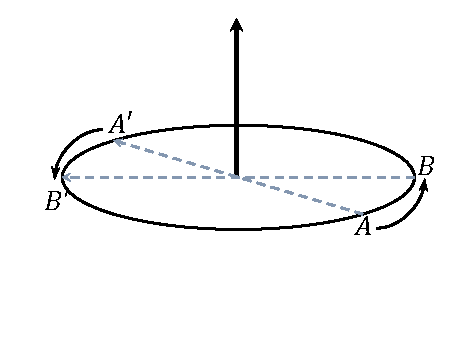
\includegraphics[width=0.6\textwidth,height=\textheight,keepaspectratio]{Seminar_08/pics/pic_01.pdf}
    \caption{Постоянство аксиального вектора при инверсии}
    \label{fig:sem_08_pic_1}
\end{figure}
Теперь скажем про знакомые нам системы, где появляется момент импульса $l$, например атом. Что тогда будет с четностью? Ответ можно получить строго, подставив известные нам решения уравнения Шредингера для случая сферически симметричного случая, это я опущу и скажу, что для такой системы $\mathfrak{p} = (-1)^l$. Если же система состоит из нескольких частей, то помимо простого произведения четности каждой из компонент этой системы, нужно учесть еще четность из относительного движения: $\mathfrak{p} = \mathfrak{p}_A\cdot\mathfrak{p}_B\cdot (-1)^{(l_A+l_B)}$. Более того, для всех типов взаимодействия, кроме слабого, работает закон сохранения четности. 
\paragraph{Золотое правило Ферми. Вероятности переходов}
Рассмотрим вот такую задачу:
\begin{equation*}
    \begin{cases}
    \hat{H_0}\psi_i=E_i\psi_i\\
    \hat{H}=\hat{H_0}+\hat{A}\xi \cos{\omega t}
    \end{cases}
\end{equation*}
Пусть у нас есть задача на поиск стационарных решений для известного оператора Гамильтона с индексом 0 и все уровни энергии $E_i$ мы знаем, тогда теперь добавим переменное по времени слабое по сравнению с остальным воздействие на систему. Это будет наше переменное поле, с которым наша система взаимодействует. Под действие такого вот воздействия система может поменять свое состояние с вероятностью:
\begin{equation*}
    \rho_{ij} \sim \left| \int \psi^*_i\hat{A}\xi\psi_j dV\right|^2 \delta (E_i-E_j \pm \hbar \omega)
\end{equation*}
Это и есть золотое правило Ферми. Дельта-функция здесь просто говорит нам о законе сохранения энергии и подборе частоты так, чтобы расстояние между известными уровнями точно соблюдалось, а вот с интегралом надо бы разобраться подробнее. Во-первых что же такое оператор $\hat{A}$ и какой смысл он в себе несет? Это оператор физической величины системы, который обеспечивает связь с переменным воздействием. Если говорить об атоме, то это может быть, например, оператор дипольного момента атома, как электрического, так и магнитного или просто заряд атома или что-то более сложное. А что это за состояния и что означает этот интеграл. Мы знаем, что i и j состояния, это собственные состояния системы и они являются независимыми. То есть получается, что наш оператор $\hat{A}$ должен <<перепутать>> наши состояния, иначе перехода не произойдет. Более того, мы можем переставить i и j местами и вероятность от этого никак не измениться. То есть неважно переход идет снизу вверх или сверху вниз.
\paragraph{Мультипольное разложение. E и M фотоны}
Теперь давайте посмотрим и запишем более подробно, какие у нас могут быть физические величины у разных систем, который взаимодействует с электромагнитным полем. Начнем с электрической составляющей. Первое, что приходит на ум, это просто записать положение каждого конкретного заряда в системе и закончить с этим. Это может быть совершенно нерационально, особенно, если мы говорим о сложном атоме, где десятки протонов и электронов, которые как-то живут вокруг ядра. Более того, не факт, что наше поле, которое взаимодействует с атомом существенно меняется с положением внутри атома. Поэтому мы можем воспользоваться трюком, который носит название "мультипольное разложение" В чем его суть? Давайте объединим все эти зарядики, которые сидят в атоме и представим их как одни -- простая сумма зарядов (скаляр $q = \sum q_i$). Это первый член такого разложения. Обычно нам везет и атом нейтрален, поэтому суммарный заряд равен 0. Но ведь атом с полем взаимодействует! Тогда можем заменить нашу систему зарядов диполем с известным положением плюса и минуса (вектор $\textbf{d} = \sum q_i \textbf{r}_i$). А вот такая штука совершенно не обязательно равна нулю. Если нам этого не хватает можем пойти дальше и сделать из зарядов квадруполь (тензор второго ранга, или проще матрица $Q_{\alpha\beta} = \sum q_i(3r_{i\alpha}r_{i\beta}-r^2\delta_{\alpha\beta}) $, см. \ref{fig:sem_08_quad}) и так далее. Тогда суммарная энергия взаимодействия с таким вот разложением:
\begin{equation*}
    \varepsilon = q\phi - (\textbf{d}\cdot\textbf{ E}) - \dfrac{1}{2}\sum Q_{\alpha\beta}\dfrac{\partial E_{\alpha}}{\partial r_{\beta}}+ \dots
\end{equation*}

\begin{figure}[h]
    \centering
    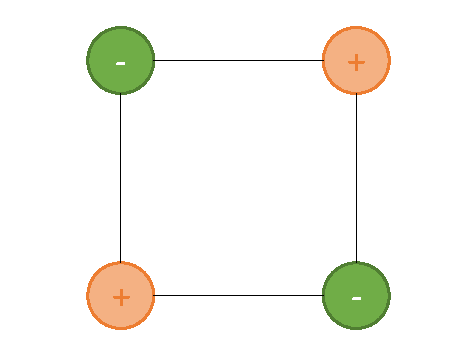
\includegraphics[width=0.4\textwidth,height=\textheight,keepaspectratio]{Seminar_08/pics/pic_02.pdf}
    \caption{Квадруполь}
    \label{fig:sem_08_quad}
\end{figure}
Для магнитного поля обычно достаточно рассмотреть магнитный момент и все, но тоже можно извратиться и двинуться в сторону квадруполей.\\
А теперь наконец давайте попытаемся сформулировать правила отбора по четности. Для этого еще раз смотрим на вероятность перехода между состояниями из золотого правила Ферми на примере электрического дипольного момента:
\begin{equation*}
    \rho_{ij} \sim \left| \int \psi^*_i\hat{d}\xi\psi_j dV\right|^2
\end{equation*}
Электрический дипольный момент это истинный вектор и при преобразовании инверсии его знак меняется на противоположенный, но ведь инверсия это просто выбор правой или левой системы координат, а природа не знает различий между ними и переход, если он возможен, будет в любой из систем. Тогда смотрим на этот интеграл и видим, что если состояния обладают одинаковой четностью к инверсии, то под интегралом стоит нечетная функция и такой интеграл равен нулю. То есть для дипольного электрического перехода необходимо изменение четности состояния. Мы уже показали, что четность определяется как $(-1)^l$, что означает что такие переходы разрешены между S и P состояниями, но запрещены между например S и S состояниями


\begin{figure}[h]
    \centering
    % 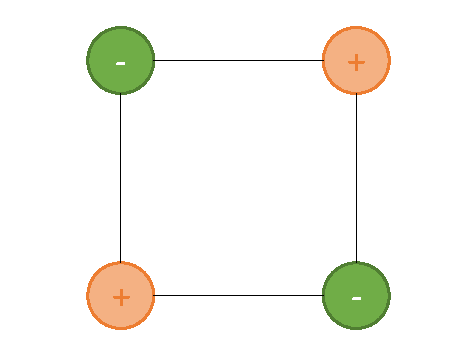
\includegraphics[width=0.4\textwidth,height=\textheight,keepaspectratio]{Seminar_08/pics/pic_02.pdf}
    \caption{Квадруполь}
    \label{fig:sem_08_quad}
\end{figure}
\section{Практическая часть}
\subsection{Задача}
\label{task_}
\paragraph{Условие}
\paragraph{Решение}

\subsection{Задача}
\label{task_}
\paragraph{Условие}
\paragraph{Решение}

\subsection{Задача}
\label{task_}
\paragraph{Условие}
\paragraph{Решение}

\subsection{Задача}
\label{task_}
\paragraph{Условие}
\paragraph{Решение}

\subsection{Задача}
\label{task_}
\paragraph{Условие}
\paragraph{Решение}

\subsection{Комментарии к задачам из задания}
\paragraph{Нулевки} 
\paragraph{Задача } 
\paragraph{Задача } 
\paragraph{Задача }
\paragraph{Задача }
\paragraph{Задача }
\paragraph{Задача }

\end{document}
